%% To get pdf-file:    (acroread below allows you to look at pdf-file)
%====================
% (A) if your figures are ps-files or eps-files  (and not pdf,png,jpeg,etc.):
%---------------------------------------------------------------------
% latex trafficflowtalk.tex ;trafficflowtalk.tex ; dvips trafficflowtalk.dvi -o ; ps2pdf trafficflowtalk.ps ; acroread trafficflowtalk.pdf
% 
% (B) if your figures are pdf,png,jpeg etc (and not ps-files or eps-files)
%---------------------------------------------------------------------
% pdflatex beamer_example.tex 
%
\documentclass[t]{beamer}
% Ben's option:
\usecolortheme{whale}       
% Sophie's option:
%\usepackage{beamerthemeBerkeley}
%
\usefonttheme[onlymath]{serif}   
\usepackage{graphicx}
\usepackage{caption}
\usepackage{braket}

\usepackage{subfig}
\usepackage{commath}

\setbeamertemplate{navigation symbols}{}  % turns off annoying nav. symbols

\title{Real Time Signal Processing with Symmetric and Asymmetric Support Intervals}
\author{Keven Joyce and Lia Harrington \\
       University of Montana}
\date{May 14, 2015}
 
% for a recurring outline
% (this defines, what happens whenever you use \section{...}, namely
%     slide is created with title "Universality ..." and table of contents
%     which includes all section titles and highlights current section)
\AtBeginSection[]  
{
\begin{frame}
\frametitle{Outline} 
\tableofcontents[currentsection] 
\end{frame}  
}

\begin{document}

%%%%%%%%%%%%%%%%%%%%%%%%%%%%%%%%%%%%%%%%%%%%%%%%%%%%%%%%%%%%%%
\begin{frame}
\titlepage
\end{frame}
%%%%%%%%%%%%%%%%%%%%%%%%%%%%%%%%%%%%%%%%%%%%%%%%%%%%%%%%%%%%%
\section{Introduction and Motivation}
%%%%%%%%%%%%%%%%%%%%%%%%%%%%%%%%%%%%%%%%%%%%%%%%%%%%%%%%%%%%%
\begin{frame}
\frametitle{Importance of Real Time Signal Processing}
\vspace{.3cm}
\structure{What is real time signal processing?}
\vspace{.3cm}
\begin{itemize}
\item Applications
\begin{itemize}
\item Speech recognition
\item Audio signal processing
\item Video compression
\item Weather forecasting
\item Economic forecasting
\item Medical imagining (e.g., CAT, MRI)
\item And more...
\end{itemize}
\end{itemize}
\end{frame}
%%%%%%%%%%%%%%%%%%%%%%%%%%%%%%%%%%%%%%%%%%%%%%%%%%%%%%%%%%%%
\section{Problem Outline}
%%%%%%%%%%%%%%%%%%%%%%%%%%%%%%%%%%%%%%%%%%%%%%%%%%%%%%%%%%%%
\begin{frame}
\frametitle{What is the problem?}
\structure{Goal:} We wish to reconstruct some generated signal $\hat{x}$ that has been distorted by some error and convolution processes. \newline \vspace{.5cm}

\structure{Solution:} Take the convolution inverse of $\hat{x}$ to reconstruct the signal. 
\end{frame}
%%%%%%%%%%%%%%%%%%%%%%%%%%%%%%%%%%%%%%%%%%%%%%%%%%%%%%%%%%%%
\section{Problem Approach and Steps} 
%%%%%%%%%%%%%%%%%%%%%%%%%%%%%%%%%%%%%%%%%%%%%%%%%%%%%%%%%%%%
\begin{frame}
\frametitle{Problem Approach Overview}
\begin{enumerate}
\item Specify problem settings
\begin{itemize}
\item $y = a*x+\nu, \hspace{.2cm} \nu ~(0,\sigma^2\delta). $
\item $ \hat{x} = r*y$ 
\begin{itemize}
\item $ r = P^{-1}q$ 
\end{itemize}
\item Choose some $\Delta = [-d,d]$  $\rightarrow $ initial estimate of $x$
\item Choose some $\Delta = [T,\tau]$  $\rightarrow $ initial estimate of $x$
\end{itemize}
\item Compute optimal $\Delta$ for $r$
\begin{itemize}
\item $H(\Delta) = E(\hat{x}_{i} - x_{i})^2 = f_{0} - \braket{q,P^-1q}\Delta$
\item Plot $H(\Delta)$ vs $d$ $\rightarrow$ optimal $d$ $\rightarrow$ optimal $r$
\end{itemize}
\item Simulation of measurement and processing
\item Illustrate the result of estimation
\begin{itemize}
\item $\sqrt{E(\hat{x}_{i} - x_{i}})^2 = \sqrt{H}$
\end{itemize}
\end{enumerate}
\end{frame}
%%%%%%%%%%%%%%%%%%%%%%%%%%%%%%%%%%%%%%%%%%%%%%%%%%%%%%%%%%%%
\begin{frame}
\frametitle{Problem Strategy: Step 1}
\structure{Specify the main ingredients of simulated measurement system:}
\begin{itemize}
\item Specify point spread function (influence function ) a, 
\begin{itemize}
\item Symmetric
\item Asymmetric
\end{itemize}
\item Covariance function $\phi$ for the signal $x$: 
\begin{equation}
\phi = Cov(x) = b*b^{*}
\end{equation}
\item Variance $\sigma^2$ of the independent components of the additive random noise $\nu$
\begin{equation}
y = a*x+\nu, \hspace{.2cm} \nu ~(0,\sigma^2\delta). 
\end{equation}
\item Choose support interval $\Delta = [-d,d] $ or $\Delta = [T,\tau]$
\end{itemize}
\end{frame}
%%%%%%%%%%%%%%%%%%%%%%%%%%%%%%%%%%%%%%%%%%%%%%%%%%%%%%%%%%%%
\begin{frame}
\frametitle{Signal and Covariance Setup}

\begin{columns}[t]
\column{.9\textwidth}
\centering
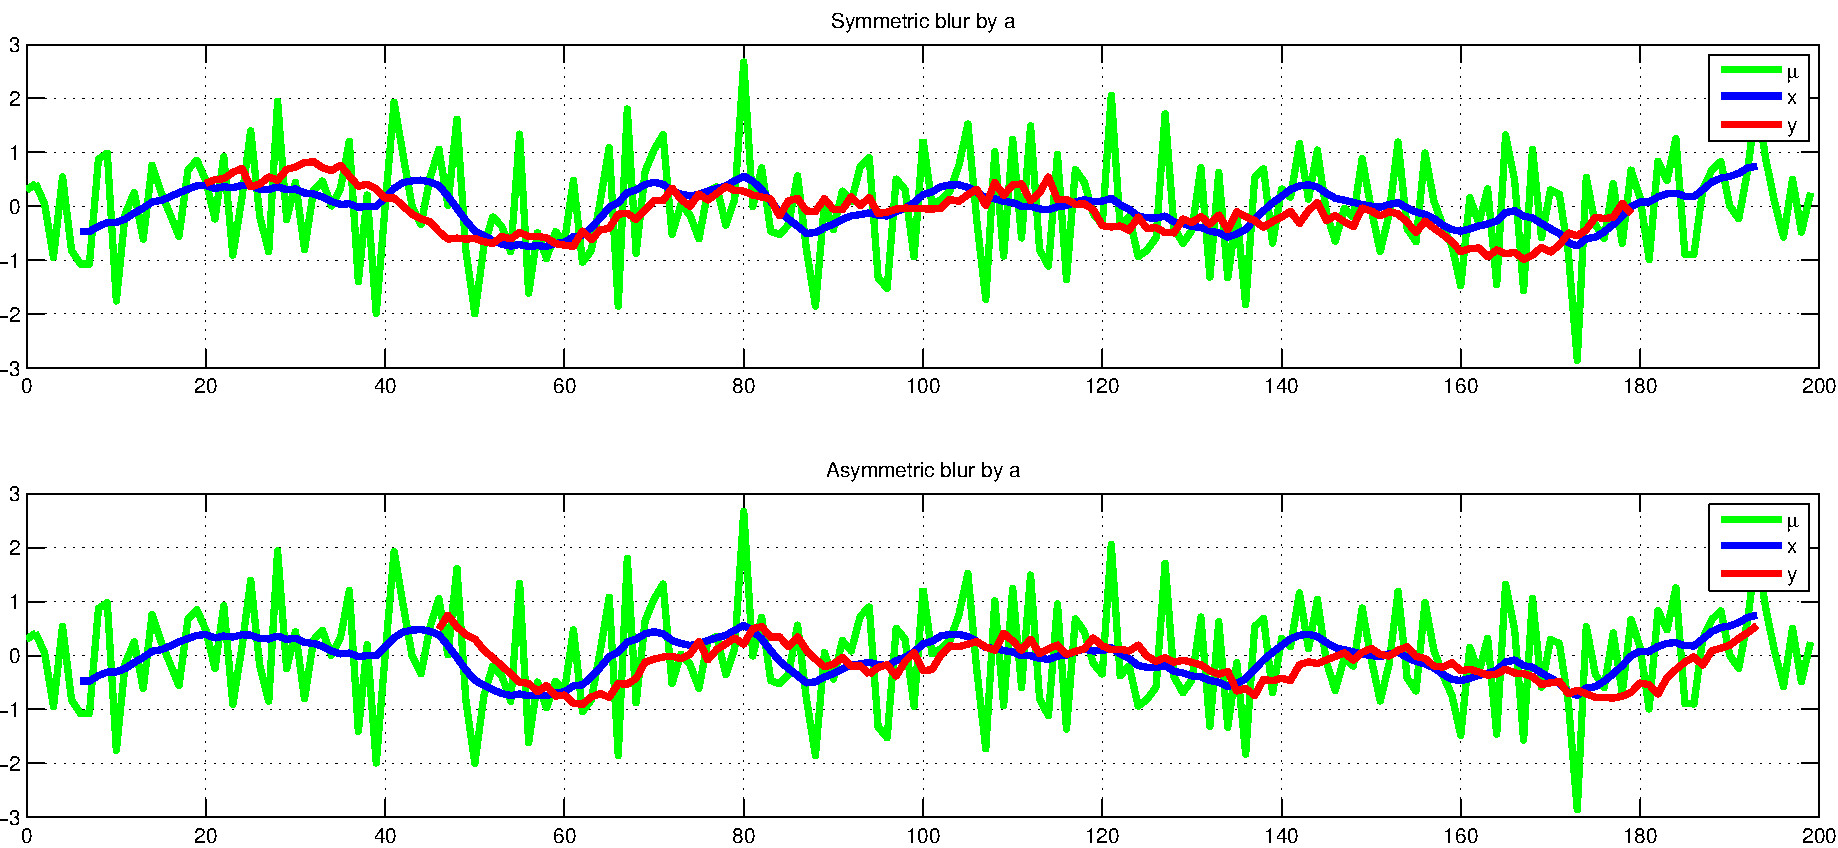
\includegraphics[scale=.3]{signal_setup.pdf}\\
%\vspace{.2cm}
%\column{.5\textwidth}
\includegraphics[scale=.3]{covariance_psf_setup.pdf}
\end{columns}

\end{frame}
%%%%%%%%%%%%%%%%%%%%%%%%%%%%%%%%%%%%%%%%%%%%%%%%%%%%%%%%%%%%
\section{Code Comments}
%%%%%%%%%%%%%%%%%%%%%%%%%%%%%%%%%%%%%%%%%%%%%%%%%%%%%%%%%%%%
\section{Results and Conclusions}
%%%%%%%%%%%%%%%%%%%%%%%%%%%%%%%%%%%%%%%%%%%%%%%%%%%%%%%%%%%%
\begin{frame}
\frametitle{References}

[1] Golubtsov, P. (2015). Theoretical Big Data Analytics course notes.

\end{frame}

\end{document}




\end{document}
